\documentclass {article}
\usepackage[margin=1.0in]{geometry}
\usepackage[style=mla-new]{biblatex}
\usepackage[hidelinks]{hyperref}
\usepackage{graphicx}
\usepackage{titlesec}
\usepackage{tikz}
\titlespacing*{\section}{0pt}{3ex plus .5ex minus .2ex}{0ex}
\addbibresource{sources.bib}
\newcommand{\sechint}[1]{\small{\emph{#1}} \bigskip}
\usepackage[acronym]{glossaries}
\makeglossaries

\begin{document}
\newacronym{scms}{SCMS}{Security Credential Management System}

\newacronym{crl}{CRL}{Certificate Revocation List}

\newacronym{rse}{RSE}{Road Side Equipment}

\newacronym{obe}{OBE}{On Board Equipment}

\newacronym{asd}{ASD}{Aftermarket Safety Device}

\newacronym{vpki}{V-PKI}{Vehicular Public Key Infrastructure}

\newacronym{vanet}{VANET}{Vehicular Ad-Hoc NETwork}

\newacronym{bsm}{BSM}{Basic Safety Message}

\newacronym{pki}{PKI}{Public Key Infrastructure}

\newacronym{v2v}{V2V}{Vehicle to Vehicle}

\newacronym{v2i}{V2I}{Vehicle to Infrastructure}

\begin{titlepage}
	\centering
	
\includegraphics[width=0.8\textwidth]{images/umd_logo.jpg} \\ \bigskip
	\LARGE{Electrical and Computer Engineering Department \\University of Massachusetts Dartmouth}\\
	\bigskip 
	\LARGE{Master's of Science \\ Thesis Proposal Update -- Third Draft} \\
	\bigskip 
	\Huge{\bf Viral Certificate Revocation List Distribution for the Security Credential Management System} \\ \medskip
	\LARGE{\bf By Robert Mushrall III}

	\vfill
	\begin{table}[!hb]
		\centering
		\begin{tabular}{ l l }
			\line(1,0){250} & \line(1,0){150} \\
			\small{Robert Mushrall III}  & \small{Date} \\
			\small{Electrical and Computer Engineering Department} \\
			\small{M.S. Computer Engineering Student} & \\
			\vspace{.3cm} \\
			\line(1,0){250} & \line(1,0){150} \\
			\small{Dr. Hong Liu} & \small{Date} \\
			\small{Electrical and Computer Engineering Department} \\
			\small{Graduate Advisor} & \\
			\vspace{.3cm} \\
			\line(1,0){250} & \line(1,0){150} \\
			\small{Dr. Paul Fortier} & \small{Date} \\
			\small{Electrical and Computer Engineering Department} \\
			\small{Graduate Committee} & \\
			\vspace{.3cm} \\
			\line(1,0){250} & \line(1,0){150} \\
			\small{Brian Hewett} & \small{Date} \\
			\small{Product Manager, General Dynamics Mission Systems} \\
			\small{Graduate Committee} & \\
		\end{tabular}
	\end{table}
	\thispagestyle{empty}
\end{titlepage}
\setcounter{page}{2}

\tableofcontents
\pagebreak

\section{Background}{\sechint{One paragraph (1/3 page) to orient the reader to the area of research.}}

With the number of vehicles on the road and the safety risks these vehicles (and their drivers) pose, new technology is needed to reduce accidents and improve travel in terms of congestion control and comfort. A \gls{vanet} will open up communication channels through the use of the \gls{bsm}, allowing helpful information to be passed between vehicles and alerting drivers of possible hazards or even adjusting routes to minimize travel time. This network will be possible with \gls{v2v} and \gls{v2i} communication. \gls{v2v}  communication allows vehicles to pass information, such as speed and nearby dangers, between each other. \gls{v2i}  communication allows vehicles to communicate with an infrastructure that may provide extra benefits to a \gls{vanet}.

While helpful information can be passed, vehicles may malfunction and attackers can cause vehicles to misbehave, which can negatively impact safety, counter to the very reason \gls{vanet} exists. The \gls{scms} is the leading solution to secure \gls{vanet} communication. It includes components common to a typical \gls{pki}, with the addition of several functions to account for the differences between a traditional network verses a \gls{vanet}. These differences come from two areas. The first is the high mobility of the network nodes. This means that routes to specific vehicles will change over time, verses a typical network where nodes are stationary for at least some period of time. The second difference is how confidentiality is maintained. Instead of keeping the contents of messages private through encryption, the identity of the sender is concealed through the use of Pseudonym Certificates. These pseudonym certificates are issued in large patches to vehicles and linking them to a single vehicle is not feasible without the use of multiple \gls{scms} components. In a typical \gls{pki} environment, a user who has been issued a certificate gets revoked by adding the issued certificate to a \gls{crl}. \gls{scms} performs a similar action when revoking a vehicle, however, the vehicle also gets added to an internal blacklist so it cannot receive new certificates.

\section{Problem Statement}{\sechint{One or two sentences that concisely state the problem that will be addressed by the research.}}

The current method for distributing \gls{crl}s is not effective for vehicles that do not have an active internet connection. A method for distributing \gls{crl}s must be defined that allows updates to be timely, does not overload the finite resource used for \gls{v2v} and \gls{v2i} communication, and provides the widest dissemination possible.

\section{Technical Discussion}{\sechint{About one page that presents some of the more important aspects of the proposed research. This should include a summary of the state-of-the-art in the particular research area.}}

\gls{scms} uses \gls{crl}s that are somewhat different than a typical \gls{crl} used in most forms of \gls{pki}. The use of pseudonym certificates, as detailed below, requires the use of linkage values to feasibly revoke devices. There is currently no permanent method in place, however research has been done previously on a collaborative distribution method.

\subsection{The Security Credential Management System}
Whyte, Weimerskirch, Kumar and Hehn propose \gls{scms}, the \gls{vpki} that this research will be focused on. This scheme is currently being finalized with the US Department of Transportation~\autocite{brecht_security_2018}. Figure~\ref{scms_overview} represents \gls{scms} as a whole, using dashed lines to represent trust, dotted lines to represent out-of-band communication, and solid lines to represent int-band or normal communication. 
\begin{figure}[!ht]
	\centering
	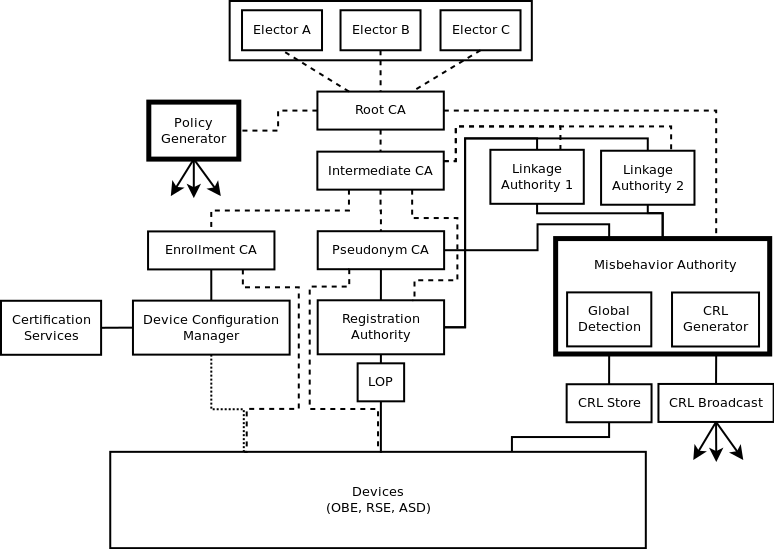
\includegraphics[width=.8\textwidth]{images/scms_diagram.png}
	\caption{\gls{scms} Overview}
	\label{scms_overview}
\end{figure}
The trust within \gls{scms} begins with the Root CA, which then trusts the Intermediate CA, the Policy Generator, and the Misbehavior Authority. In turn, the Intermediate CA trusts the Enrollment CA, the Pseudonym CA, the Registration Authority, and the linkage authorities. The end devices, such as the \gls{obe}, \gls{rse} and \gls{asd}, are all trusted by the Enrollment CA and the Pseudonym CA. The electors are part of \gls{scms}'s self-healing function. They vote to endorse or reject the Root CA, allowing a new Root CA to be voted in. In the event the Root CA's private key is compromised or expired, the electors will vote on the new Root CA, and all necessary components and end devices will update their trust. The Policy Generator and the Misbehavior Authority are intrinsically central (bold), meaning that only one of these must exist for \gls{scms} to function properly.

There are four main use cases with \gls{scms}: device bootstrapping, certificate provisioning, misbehavior reporting, and global misbehavior detection and revocation~\autocite{brecht_security_2018}. Device bootstrapping is the process of initializing the device so it may authenticate itself to \gls{scms}. First, all the necessary certificates needed to communicate with \gls{scms} are loaded onto the device, such as the Certificate Authorities, the Misbehavior Authority, and the Registration Authority. Next, it gets an enrollment certificate which can be used to communicate with \gls{scms}. Certificate provisioning is the process of providing pseudonym certificates to the device so that it may communicate with other devices anonymously. Misbehavior reporting is the process that vehicles submit reports of misbehaving vehicles to the Misbehavior Authority. Vehicles will have local misbehavior detection, while \gls{scms} will have global misbehavior algorithms that utilize misbehavior reports that vehicles provide. This global misbehavior detection and revocation will involve collecting misbehavior reports, determine the devices using the linkage authorities, and revoke the device. Revoking a device involves adding the device to an internal blacklist so that it may not be provisioned new pseudonym certificates, as well as adding the device to the \gls{crl}, so it may be distributed to other devices.

\subsection{CRLs in SCMS}
Pseudonym certificates make privacy possible in \gls{scms}, however it becomes a nightmare to revoke all certificates associated with one device. Each device will receive enough certificates for twenty to be valid per week, for anywhere between one and three years~\autocite{brecht_security_2018}, meaning roughly 3,000 certificates will need to be revoked for just one device. This problem was solved with linkage values. For each batch of pseudonym certificates, linkage values will be generated and included in the certificates. This means only one number is needed to revoke all pseudonym certificates, making \gls{crl}s feasible in \gls{scms}.

\subsection{State of the Art}
Currently, \gls{crl}s are distributed via an HTTP GET request to an online server~\autocite{brecht_scms_nodate}, however \autocite{brecht_security_2018} state that a \gls{crl} distribution method based on collaborative distribution, proposed by \autocite{haas_efficient_2011} needs to be defined. This paper makes several suggestions as to make revoking pseudonym certificates feasible, which are similar to the solutions that \gls{scms} plan to implement, as well as outline their method for distributing \gls{crl}s. Their method involves a few \gls{rse}s broadcasting the current \gls{crl} to vehicles, then have the vehicles broadcast the \gls{crl} to other vehicles. They demonstrate their approach by using a custom simulator accounting for the area surrounding Zurich, Switzerland with roughly 260,000 vehicles, and measured the number of vehicles with the \gls{crl} after initially distributing it~\autocite{haas_efficient_2011}.

\section{Approach}{\sechint{One paragraph (1/3 page) that describes the methods that will be applied in conducting the research.}}

An initial design has been drafted and is detailed below. The proposed solution will be tested in simulation on its ability to distribute changing \gls{crl}s .

\subsection{Solution: Viral CRL Distribution}
This proposed method will effectively distribute \gls{crl}s much like a virus; a few \gls{rse}s will ``infect'' nearby vehicles with the current \gls{crl}, who will then infect other vehicles with the current \gls{crl}. To make this feasible for a changing \gls{crl}, extra measures will take place. The first is to break the list into segments. Each segment will be signed by the Misbehavior Authority to ensure integrity, versioned in sequential order, and include an expiration date. The second is to include a second list, as detailed below. Additional measures will be worked out during simulation.

\begin{figure}[!ht]
	\centering
	% Graphic for TeX using PGF
% Title: /home/robert/school/ThesisResearch/src_proposal/incr_update.dia
% Creator: Dia v0.97.3
% CreationDate: Sat Jun  2 08:49:05 2018
% For: robert
% \usepackage{tikz}
% The following commands are not supported in PSTricks at present
% We define them conditionally, so when they are implemented,
% this pgf file will use them.
\ifx\du\undefined
  \newlength{\du}
\fi
\setlength{\du}{15\unitlength}
\begin{tikzpicture}
\pgftransformxscale{1.000000}
\pgftransformyscale{-1.000000}
\definecolor{dialinecolor}{rgb}{0.000000, 0.000000, 0.000000}
\pgfsetstrokecolor{dialinecolor}
\definecolor{dialinecolor}{rgb}{1.000000, 1.000000, 1.000000}
\pgfsetfillcolor{dialinecolor}
\definecolor{dialinecolor}{rgb}{1.000000, 1.000000, 1.000000}
\pgfsetfillcolor{dialinecolor}
\fill (5.061250\du,4.950000\du)--(5.061250\du,7.650000\du)--(7.923750\du,7.650000\du)--(7.923750\du,4.950000\du)--cycle;
\pgfsetlinewidth{0.100000\du}
\pgfsetdash{}{0pt}
\pgfsetdash{}{0pt}
\pgfsetmiterjoin
\definecolor{dialinecolor}{rgb}{0.000000, 0.000000, 0.000000}
\pgfsetstrokecolor{dialinecolor}
\draw (5.061250\du,4.950000\du)--(5.061250\du,7.650000\du)--(7.923750\du,7.650000\du)--(7.923750\du,4.950000\du)--cycle;
% setfont left to latex
\definecolor{dialinecolor}{rgb}{0.000000, 0.000000, 0.000000}
\pgfsetstrokecolor{dialinecolor}
\node at (6.492500\du,6.095000\du){CRL:};
% setfont left to latex
\definecolor{dialinecolor}{rgb}{0.000000, 0.000000, 0.000000}
\pgfsetstrokecolor{dialinecolor}
\node at (6.492500\du,6.895000\du){Cert1};
\definecolor{dialinecolor}{rgb}{1.000000, 1.000000, 1.000000}
\pgfsetfillcolor{dialinecolor}
\fill (12.065000\du,5.005000\du)--(12.065000\du,8.505000\du)--(15.142500\du,8.505000\du)--(15.142500\du,5.005000\du)--cycle;
\pgfsetlinewidth{0.100000\du}
\pgfsetdash{}{0pt}
\pgfsetdash{}{0pt}
\pgfsetmiterjoin
\definecolor{dialinecolor}{rgb}{0.000000, 0.000000, 0.000000}
\pgfsetstrokecolor{dialinecolor}
\draw (12.065000\du,5.005000\du)--(12.065000\du,8.505000\du)--(15.142500\du,8.505000\du)--(15.142500\du,5.005000\du)--cycle;
% setfont left to latex
\definecolor{dialinecolor}{rgb}{0.000000, 0.000000, 0.000000}
\pgfsetstrokecolor{dialinecolor}
\node at (13.603750\du,6.150000\du){CRL:};
% setfont left to latex
\definecolor{dialinecolor}{rgb}{0.000000, 0.000000, 0.000000}
\pgfsetstrokecolor{dialinecolor}
\node at (13.603750\du,6.950000\du){Cert1};
% setfont left to latex
\definecolor{dialinecolor}{rgb}{0.000000, 0.000000, 0.000000}
\pgfsetstrokecolor{dialinecolor}
\node at (13.603750\du,7.750000\du){Cert2};
\pgfsetlinewidth{0.100000\du}
\pgfsetdash{}{0pt}
\pgfsetdash{}{0pt}
\pgfsetbuttcap
\pgfsetmiterjoin
\pgfsetlinewidth{0.100000\du}
\pgfsetbuttcap
\pgfsetmiterjoin
\pgfsetdash{}{0pt}
\definecolor{dialinecolor}{rgb}{1.000000, 1.000000, 1.000000}
\pgfsetfillcolor{dialinecolor}
\fill (8.950000\du,6.037500\du)--(10.025000\du,6.037500\du)--(10.383333\du,6.037500\du)--(10.383333\du,5.550000\du)--(11.100000\du,6.525000\du)--(10.383333\du,7.500000\du)--(10.383333\du,7.012500\du)--(8.950000\du,7.012500\du)--cycle;
\definecolor{dialinecolor}{rgb}{0.000000, 0.000000, 0.000000}
\pgfsetstrokecolor{dialinecolor}
\draw (8.950000\du,6.037500\du)--(10.025000\du,6.037500\du)--(10.383333\du,6.037500\du)--(10.383333\du,5.550000\du)--(11.100000\du,6.525000\du)--(10.383333\du,7.500000\du)--(10.383333\du,7.012500\du)--(8.950000\du,7.012500\du)--cycle;
\pgfsetbuttcap
\pgfsetmiterjoin
\pgfsetdash{}{0pt}
\definecolor{dialinecolor}{rgb}{0.000000, 0.000000, 0.000000}
\pgfsetstrokecolor{dialinecolor}
\draw (8.950000\du,6.037500\du)--(10.025000\du,6.037500\du)--(10.383333\du,6.037500\du)--(10.383333\du,5.550000\du)--(11.100000\du,6.525000\du)--(10.383333\du,7.500000\du)--(10.383333\du,7.012500\du)--(8.950000\du,7.012500\du)--cycle;
\definecolor{dialinecolor}{rgb}{1.000000, 1.000000, 1.000000}
\pgfsetfillcolor{dialinecolor}
\fill (19.165000\du,5.005000\du)--(19.165000\du,9.305000\du)--(22.242500\du,9.305000\du)--(22.242500\du,5.005000\du)--cycle;
\pgfsetlinewidth{0.100000\du}
\pgfsetdash{}{0pt}
\pgfsetdash{}{0pt}
\pgfsetmiterjoin
\definecolor{dialinecolor}{rgb}{0.000000, 0.000000, 0.000000}
\pgfsetstrokecolor{dialinecolor}
\draw (19.165000\du,5.005000\du)--(19.165000\du,9.305000\du)--(22.242500\du,9.305000\du)--(22.242500\du,5.005000\du)--cycle;
% setfont left to latex
\definecolor{dialinecolor}{rgb}{0.000000, 0.000000, 0.000000}
\pgfsetstrokecolor{dialinecolor}
\node at (20.703750\du,6.150000\du){CRL:};
% setfont left to latex
\definecolor{dialinecolor}{rgb}{0.000000, 0.000000, 0.000000}
\pgfsetstrokecolor{dialinecolor}
\node at (20.703750\du,6.950000\du){Cert1};
% setfont left to latex
\definecolor{dialinecolor}{rgb}{0.000000, 0.000000, 0.000000}
\pgfsetstrokecolor{dialinecolor}
\node at (20.703750\du,7.750000\du){Cert2};
% setfont left to latex
\definecolor{dialinecolor}{rgb}{0.000000, 0.000000, 0.000000}
\pgfsetstrokecolor{dialinecolor}
\node at (20.703750\du,8.550000\du){Cert3};
\pgfsetlinewidth{0.100000\du}
\pgfsetdash{}{0pt}
\pgfsetdash{}{0pt}
\pgfsetbuttcap
\pgfsetmiterjoin
\pgfsetlinewidth{0.100000\du}
\pgfsetbuttcap
\pgfsetmiterjoin
\pgfsetdash{}{0pt}
\definecolor{dialinecolor}{rgb}{1.000000, 1.000000, 1.000000}
\pgfsetfillcolor{dialinecolor}
\fill (16.165000\du,6.044946\du)--(17.240000\du,6.044946\du)--(17.598333\du,6.044946\du)--(17.598333\du,5.557446\du)--(18.315000\du,6.532446\du)--(17.598333\du,7.507446\du)--(17.598333\du,7.019946\du)--(16.165000\du,7.019946\du)--cycle;
\definecolor{dialinecolor}{rgb}{0.000000, 0.000000, 0.000000}
\pgfsetstrokecolor{dialinecolor}
\draw (16.165000\du,6.044946\du)--(17.240000\du,6.044946\du)--(17.598333\du,6.044946\du)--(17.598333\du,5.557446\du)--(18.315000\du,6.532446\du)--(17.598333\du,7.507446\du)--(17.598333\du,7.019946\du)--(16.165000\du,7.019946\du)--cycle;
\pgfsetbuttcap
\pgfsetmiterjoin
\pgfsetdash{}{0pt}
\definecolor{dialinecolor}{rgb}{0.000000, 0.000000, 0.000000}
\pgfsetstrokecolor{dialinecolor}
\draw (16.165000\du,6.044946\du)--(17.240000\du,6.044946\du)--(17.598333\du,6.044946\du)--(17.598333\du,5.557446\du)--(18.315000\du,6.532446\du)--(17.598333\du,7.507446\du)--(17.598333\du,7.019946\du)--(16.165000\du,7.019946\du)--cycle;
\pgfsetlinewidth{0.100000\du}
\pgfsetdash{}{0pt}
\pgfsetdash{}{0pt}
\pgfsetbuttcap
\pgfsetmiterjoin
\pgfsetlinewidth{0.100000\du}
\pgfsetbuttcap
\pgfsetmiterjoin
\pgfsetdash{}{0pt}
\definecolor{dialinecolor}{rgb}{1.000000, 1.000000, 1.000000}
\pgfsetfillcolor{dialinecolor}
\fill (23.315000\du,6.494946\du)--(24.390000\du,6.494946\du)--(24.748333\du,6.494946\du)--(24.748333\du,6.007446\du)--(25.465000\du,6.982446\du)--(24.748333\du,7.957446\du)--(24.748333\du,7.469946\du)--(23.315000\du,7.469946\du)--cycle;
\definecolor{dialinecolor}{rgb}{0.000000, 0.000000, 0.000000}
\pgfsetstrokecolor{dialinecolor}
\draw (23.315000\du,6.494946\du)--(24.390000\du,6.494946\du)--(24.748333\du,6.494946\du)--(24.748333\du,6.007446\du)--(25.465000\du,6.982446\du)--(24.748333\du,7.957446\du)--(24.748333\du,7.469946\du)--(23.315000\du,7.469946\du)--cycle;
\pgfsetbuttcap
\pgfsetmiterjoin
\pgfsetdash{}{0pt}
\definecolor{dialinecolor}{rgb}{0.000000, 0.000000, 0.000000}
\pgfsetstrokecolor{dialinecolor}
\draw (23.315000\du,6.494946\du)--(24.390000\du,6.494946\du)--(24.748333\du,6.494946\du)--(24.748333\du,6.007446\du)--(25.465000\du,6.982446\du)--(24.748333\du,7.957446\du)--(24.748333\du,7.469946\du)--(23.315000\du,7.469946\du)--cycle;
\pgfsetlinewidth{0.100000\du}
\pgfsetdash{}{0pt}
\pgfsetdash{}{0pt}
\pgfsetbuttcap
\pgfsetmiterjoin
\pgfsetlinewidth{0.100000\du}
\pgfsetbuttcap
\pgfsetmiterjoin
\pgfsetdash{}{0pt}
\definecolor{dialinecolor}{rgb}{1.000000, 1.000000, 1.000000}
\pgfsetfillcolor{dialinecolor}
\fill (26.107813\du,5.050000\du)--(26.107813\du,10.150000\du)--(30.392188\du,10.150000\du)--(30.392188\du,5.050000\du)--cycle;
\definecolor{dialinecolor}{rgb}{0.000000, 0.000000, 0.000000}
\pgfsetstrokecolor{dialinecolor}
\draw (26.107813\du,5.050000\du)--(26.107813\du,10.150000\du)--(30.392188\du,10.150000\du)--(30.392188\du,5.050000\du)--cycle;
\pgfsetbuttcap
\pgfsetmiterjoin
\pgfsetdash{}{0pt}
\definecolor{dialinecolor}{rgb}{0.000000, 0.000000, 0.000000}
\pgfsetstrokecolor{dialinecolor}
\draw (26.536250\du,5.050000\du)--(26.536250\du,10.150000\du);
\pgfsetbuttcap
\pgfsetmiterjoin
\pgfsetdash{}{0pt}
\definecolor{dialinecolor}{rgb}{0.000000, 0.000000, 0.000000}
\pgfsetstrokecolor{dialinecolor}
\draw (29.963750\du,5.050000\du)--(29.963750\du,10.150000\du);
% setfont left to latex
\definecolor{dialinecolor}{rgb}{0.000000, 0.000000, 0.000000}
\pgfsetstrokecolor{dialinecolor}
\node at (28.250000\du,5.800000\du){Seg 1:};
% setfont left to latex
\definecolor{dialinecolor}{rgb}{0.000000, 0.000000, 0.000000}
\pgfsetstrokecolor{dialinecolor}
\node at (28.250000\du,6.600000\du){Cert1};
% setfont left to latex
\definecolor{dialinecolor}{rgb}{0.000000, 0.000000, 0.000000}
\pgfsetstrokecolor{dialinecolor}
\node at (28.250000\du,7.400000\du){Cert2};
% setfont left to latex
\definecolor{dialinecolor}{rgb}{0.000000, 0.000000, 0.000000}
\pgfsetstrokecolor{dialinecolor}
\node at (28.250000\du,8.200000\du){Cert3};
% setfont left to latex
\definecolor{dialinecolor}{rgb}{0.000000, 0.000000, 0.000000}
\pgfsetstrokecolor{dialinecolor}
\node at (28.250000\du,9.000000\du){Cert4};
% setfont left to latex
\definecolor{dialinecolor}{rgb}{0.000000, 0.000000, 0.000000}
\pgfsetstrokecolor{dialinecolor}
\node at (28.250000\du,9.800000\du){Exp. Date};
\definecolor{dialinecolor}{rgb}{1.000000, 1.000000, 1.000000}
\pgfsetfillcolor{dialinecolor}
\fill (5.065000\du,10.055000\du)--(5.065000\du,12.755000\du)--(7.927500\du,12.755000\du)--(7.927500\du,10.055000\du)--cycle;
\pgfsetlinewidth{0.100000\du}
\pgfsetdash{}{0pt}
\pgfsetdash{}{0pt}
\pgfsetmiterjoin
\definecolor{dialinecolor}{rgb}{0.000000, 0.000000, 0.000000}
\pgfsetstrokecolor{dialinecolor}
\draw (5.065000\du,10.055000\du)--(5.065000\du,12.755000\du)--(7.927500\du,12.755000\du)--(7.927500\du,10.055000\du)--cycle;
% setfont left to latex
\definecolor{dialinecolor}{rgb}{0.000000, 0.000000, 0.000000}
\pgfsetstrokecolor{dialinecolor}
\node at (6.496250\du,11.200000\du){CRL:};
% setfont left to latex
\definecolor{dialinecolor}{rgb}{0.000000, 0.000000, 0.000000}
\pgfsetstrokecolor{dialinecolor}
\node at (6.496250\du,12.000000\du){Cert5};
\definecolor{dialinecolor}{rgb}{1.000000, 1.000000, 1.000000}
\pgfsetfillcolor{dialinecolor}
\fill (12.068750\du,10.110000\du)--(12.068750\du,13.610000\du)--(15.146250\du,13.610000\du)--(15.146250\du,10.110000\du)--cycle;
\pgfsetlinewidth{0.100000\du}
\pgfsetdash{}{0pt}
\pgfsetdash{}{0pt}
\pgfsetmiterjoin
\definecolor{dialinecolor}{rgb}{0.000000, 0.000000, 0.000000}
\pgfsetstrokecolor{dialinecolor}
\draw (12.068750\du,10.110000\du)--(12.068750\du,13.610000\du)--(15.146250\du,13.610000\du)--(15.146250\du,10.110000\du)--cycle;
% setfont left to latex
\definecolor{dialinecolor}{rgb}{0.000000, 0.000000, 0.000000}
\pgfsetstrokecolor{dialinecolor}
\node at (13.607500\du,11.255000\du){CRL:};
% setfont left to latex
\definecolor{dialinecolor}{rgb}{0.000000, 0.000000, 0.000000}
\pgfsetstrokecolor{dialinecolor}
\node at (13.607500\du,12.055000\du){Cert5};
% setfont left to latex
\definecolor{dialinecolor}{rgb}{0.000000, 0.000000, 0.000000}
\pgfsetstrokecolor{dialinecolor}
\node at (13.607500\du,12.855000\du){Cert6};
\pgfsetlinewidth{0.100000\du}
\pgfsetdash{}{0pt}
\pgfsetdash{}{0pt}
\pgfsetbuttcap
\pgfsetmiterjoin
\pgfsetlinewidth{0.100000\du}
\pgfsetbuttcap
\pgfsetmiterjoin
\pgfsetdash{}{0pt}
\definecolor{dialinecolor}{rgb}{1.000000, 1.000000, 1.000000}
\pgfsetfillcolor{dialinecolor}
\fill (8.953750\du,11.142500\du)--(10.028750\du,11.142500\du)--(10.387083\du,11.142500\du)--(10.387083\du,10.655000\du)--(11.103750\du,11.630000\du)--(10.387083\du,12.605000\du)--(10.387083\du,12.117500\du)--(8.953750\du,12.117500\du)--cycle;
\definecolor{dialinecolor}{rgb}{0.000000, 0.000000, 0.000000}
\pgfsetstrokecolor{dialinecolor}
\draw (8.953750\du,11.142500\du)--(10.028750\du,11.142500\du)--(10.387083\du,11.142500\du)--(10.387083\du,10.655000\du)--(11.103750\du,11.630000\du)--(10.387083\du,12.605000\du)--(10.387083\du,12.117500\du)--(8.953750\du,12.117500\du)--cycle;
\pgfsetbuttcap
\pgfsetmiterjoin
\pgfsetdash{}{0pt}
\definecolor{dialinecolor}{rgb}{0.000000, 0.000000, 0.000000}
\pgfsetstrokecolor{dialinecolor}
\draw (8.953750\du,11.142500\du)--(10.028750\du,11.142500\du)--(10.387083\du,11.142500\du)--(10.387083\du,10.655000\du)--(11.103750\du,11.630000\du)--(10.387083\du,12.605000\du)--(10.387083\du,12.117500\du)--(8.953750\du,12.117500\du)--cycle;
\definecolor{dialinecolor}{rgb}{1.000000, 1.000000, 1.000000}
\pgfsetfillcolor{dialinecolor}
\fill (19.168750\du,10.110000\du)--(19.168750\du,14.410000\du)--(22.246250\du,14.410000\du)--(22.246250\du,10.110000\du)--cycle;
\pgfsetlinewidth{0.100000\du}
\pgfsetdash{}{0pt}
\pgfsetdash{}{0pt}
\pgfsetmiterjoin
\definecolor{dialinecolor}{rgb}{0.000000, 0.000000, 0.000000}
\pgfsetstrokecolor{dialinecolor}
\draw (19.168750\du,10.110000\du)--(19.168750\du,14.410000\du)--(22.246250\du,14.410000\du)--(22.246250\du,10.110000\du)--cycle;
% setfont left to latex
\definecolor{dialinecolor}{rgb}{0.000000, 0.000000, 0.000000}
\pgfsetstrokecolor{dialinecolor}
\node at (20.707500\du,11.255000\du){CRL:};
% setfont left to latex
\definecolor{dialinecolor}{rgb}{0.000000, 0.000000, 0.000000}
\pgfsetstrokecolor{dialinecolor}
\node at (20.707500\du,12.055000\du){Cert5};
% setfont left to latex
\definecolor{dialinecolor}{rgb}{0.000000, 0.000000, 0.000000}
\pgfsetstrokecolor{dialinecolor}
\node at (20.707500\du,12.855000\du){Cert6};
% setfont left to latex
\definecolor{dialinecolor}{rgb}{0.000000, 0.000000, 0.000000}
\pgfsetstrokecolor{dialinecolor}
\node at (20.707500\du,13.655000\du){Cert7};
\pgfsetlinewidth{0.100000\du}
\pgfsetdash{}{0pt}
\pgfsetdash{}{0pt}
\pgfsetbuttcap
\pgfsetmiterjoin
\pgfsetlinewidth{0.100000\du}
\pgfsetbuttcap
\pgfsetmiterjoin
\pgfsetdash{}{0pt}
\definecolor{dialinecolor}{rgb}{1.000000, 1.000000, 1.000000}
\pgfsetfillcolor{dialinecolor}
\fill (16.168750\du,11.149946\du)--(17.243750\du,11.149946\du)--(17.602083\du,11.149946\du)--(17.602083\du,10.662446\du)--(18.318750\du,11.637446\du)--(17.602083\du,12.612446\du)--(17.602083\du,12.124946\du)--(16.168750\du,12.124946\du)--cycle;
\definecolor{dialinecolor}{rgb}{0.000000, 0.000000, 0.000000}
\pgfsetstrokecolor{dialinecolor}
\draw (16.168750\du,11.149946\du)--(17.243750\du,11.149946\du)--(17.602083\du,11.149946\du)--(17.602083\du,10.662446\du)--(18.318750\du,11.637446\du)--(17.602083\du,12.612446\du)--(17.602083\du,12.124946\du)--(16.168750\du,12.124946\du)--cycle;
\pgfsetbuttcap
\pgfsetmiterjoin
\pgfsetdash{}{0pt}
\definecolor{dialinecolor}{rgb}{0.000000, 0.000000, 0.000000}
\pgfsetstrokecolor{dialinecolor}
\draw (16.168750\du,11.149946\du)--(17.243750\du,11.149946\du)--(17.602083\du,11.149946\du)--(17.602083\du,10.662446\du)--(18.318750\du,11.637446\du)--(17.602083\du,12.612446\du)--(17.602083\du,12.124946\du)--(16.168750\du,12.124946\du)--cycle;
\pgfsetlinewidth{0.100000\du}
\pgfsetdash{}{0pt}
\pgfsetdash{}{0pt}
\pgfsetbuttcap
\pgfsetmiterjoin
\pgfsetlinewidth{0.100000\du}
\pgfsetbuttcap
\pgfsetmiterjoin
\pgfsetdash{}{0pt}
\definecolor{dialinecolor}{rgb}{1.000000, 1.000000, 1.000000}
\pgfsetfillcolor{dialinecolor}
\fill (23.318750\du,11.599946\du)--(24.393750\du,11.599946\du)--(24.752083\du,11.599946\du)--(24.752083\du,11.112446\du)--(25.468750\du,12.087446\du)--(24.752083\du,13.062446\du)--(24.752083\du,12.574946\du)--(23.318750\du,12.574946\du)--cycle;
\definecolor{dialinecolor}{rgb}{0.000000, 0.000000, 0.000000}
\pgfsetstrokecolor{dialinecolor}
\draw (23.318750\du,11.599946\du)--(24.393750\du,11.599946\du)--(24.752083\du,11.599946\du)--(24.752083\du,11.112446\du)--(25.468750\du,12.087446\du)--(24.752083\du,13.062446\du)--(24.752083\du,12.574946\du)--(23.318750\du,12.574946\du)--cycle;
\pgfsetbuttcap
\pgfsetmiterjoin
\pgfsetdash{}{0pt}
\definecolor{dialinecolor}{rgb}{0.000000, 0.000000, 0.000000}
\pgfsetstrokecolor{dialinecolor}
\draw (23.318750\du,11.599946\du)--(24.393750\du,11.599946\du)--(24.752083\du,11.599946\du)--(24.752083\du,11.112446\du)--(25.468750\du,12.087446\du)--(24.752083\du,13.062446\du)--(24.752083\du,12.574946\du)--(23.318750\du,12.574946\du)--cycle;
\pgfsetlinewidth{0.100000\du}
\pgfsetdash{}{0pt}
\pgfsetdash{}{0pt}
\pgfsetbuttcap
\pgfsetmiterjoin
\pgfsetlinewidth{0.100000\du}
\pgfsetbuttcap
\pgfsetmiterjoin
\pgfsetdash{}{0pt}
\definecolor{dialinecolor}{rgb}{1.000000, 1.000000, 1.000000}
\pgfsetfillcolor{dialinecolor}
\fill (26.111563\du,10.155000\du)--(26.111563\du,15.255000\du)--(30.395938\du,15.255000\du)--(30.395938\du,10.155000\du)--cycle;
\definecolor{dialinecolor}{rgb}{0.000000, 0.000000, 0.000000}
\pgfsetstrokecolor{dialinecolor}
\draw (26.111563\du,10.155000\du)--(26.111563\du,15.255000\du)--(30.395938\du,15.255000\du)--(30.395938\du,10.155000\du)--cycle;
\pgfsetbuttcap
\pgfsetmiterjoin
\pgfsetdash{}{0pt}
\definecolor{dialinecolor}{rgb}{0.000000, 0.000000, 0.000000}
\pgfsetstrokecolor{dialinecolor}
\draw (26.540000\du,10.155000\du)--(26.540000\du,15.255000\du);
\pgfsetbuttcap
\pgfsetmiterjoin
\pgfsetdash{}{0pt}
\definecolor{dialinecolor}{rgb}{0.000000, 0.000000, 0.000000}
\pgfsetstrokecolor{dialinecolor}
\draw (29.967500\du,10.155000\du)--(29.967500\du,15.255000\du);
% setfont left to latex
\definecolor{dialinecolor}{rgb}{0.000000, 0.000000, 0.000000}
\pgfsetstrokecolor{dialinecolor}
\node at (28.253750\du,10.905000\du){Seg 2:};
% setfont left to latex
\definecolor{dialinecolor}{rgb}{0.000000, 0.000000, 0.000000}
\pgfsetstrokecolor{dialinecolor}
\node at (28.253750\du,11.705000\du){Cert5};
% setfont left to latex
\definecolor{dialinecolor}{rgb}{0.000000, 0.000000, 0.000000}
\pgfsetstrokecolor{dialinecolor}
\node at (28.253750\du,12.505000\du){Cert6};
% setfont left to latex
\definecolor{dialinecolor}{rgb}{0.000000, 0.000000, 0.000000}
\pgfsetstrokecolor{dialinecolor}
\node at (28.253750\du,13.305000\du){Cert7};
% setfont left to latex
\definecolor{dialinecolor}{rgb}{0.000000, 0.000000, 0.000000}
\pgfsetstrokecolor{dialinecolor}
\node at (28.253750\du,14.105000\du){Cert8};
% setfont left to latex
\definecolor{dialinecolor}{rgb}{0.000000, 0.000000, 0.000000}
\pgfsetstrokecolor{dialinecolor}
\node at (28.253750\du,14.905000\du){Exp. Date};
% setfont left to latex
\definecolor{dialinecolor}{rgb}{0.000000, 0.000000, 0.000000}
\pgfsetstrokecolor{dialinecolor}
\node[anchor=west] at (4.950000\du,4.450000\du){Delta Lists};
% setfont left to latex
\definecolor{dialinecolor}{rgb}{0.000000, 0.000000, 0.000000}
\pgfsetstrokecolor{dialinecolor}
\node[anchor=west] at (25.900000\du,4.650000\du){Permanent List};
\end{tikzpicture}

	\caption{Incremental Update}
	\label{fig:incr_update}
\end{figure}

The current proposed method will be an updated version of what was proposed by \autocite{haas_efficient_2011}. The current \gls{crl} will be broken into two lists: a permanent list, and a delta list. The \gls{crl} begins as a delta list with one entry, shown in Figure~\ref{fig:incr_update}, which gets proadcasted to devices. As new certificates get added to the list, the updated list gets distributed with an updated time stamp, until it reaches a predetermined size, four in the case of this figure. When it reaches a predetermined size, it becomes a segment in a permanent list and gets distributed with the segment number. When another certificate gets added to the \gls{crl}, it gets added to a new delta list, which will continue to grow until the predetermined size. At this point, it will become the next segment. Each delta list and segment will be signed by the Misbehavior Authority so the authenticity of the sending vehicle should not need to be verified, only the \gls{crl} itself. The latest version each vehicle has should be broadcasted in each \gls{bsm} so if a listening vehicle notices another vehicle does not have the latest update, it should broadcast the latest segment of the \gls{crl}. An alternative to this approach is for an out-of-date vehicle to request a \gls{crl} segment when it ``hears'' a vehicle with a later \gls{crl} segment. The delta list will be time-stamped and signed by the Misbehavior Authority, with the date broadcasted in the \gls{bsm} so listening vehicles can update out-of-date vehicles. Specific details of implementation will be worked out during simulation.

\subsection{Methodology}
The method proposed in \autocite{haas_efficient_2011} will be updated for use with the current policies in \gls{scms} and will account for a changing \gls{crl}. This updated method will be evaluated using Veins (v4.6), OMNeT++(v5.1), and SUMO (v0.30). OMNeT++ is a network simulator that will be used to simulate the vehicles and \gls{rse}s, where the proposed \gls{crl} distribution method will reside. SUMO is a road traffic simulator which will be used to simulate movement of vehicles. Veins is a framework that will be used to tie OMNeT++ and SUMO together. Simulations will serve two purposes: to debug and fine tune the resulting method, and to evaluate its effectiveness. This method will be evaluated on the number of vehicles with the updated \gls{crl}, similarly to the results in \autocite{haas_efficient_2011}, how continuous updates are handled, and its ability to handle large updates.

\subsection{Validation}
This research will be limited to simulations performed in software. Experiments will be considered out of scope as it is not feasible. This research will focus on the ability of changing \gls{crl}s to be distributed effectively in a simulated environment. (kind of stumped here...)

\subsection{Potential Contribution}
This research will fill a void in the current implementation of \gls{scms} by providing a flexible and dependable distribution method for \gls{crl}s that does not require vehicles to maintain an active connection to the internet. This proposed solution adds to the contribution from \autocite{haas_efficient_2011} by adding mechanisms to account for a \gls{crl} too large to be broadcasted, a changing list, and the need to keep \gls{crl}s secure.

\pagebreak
\section{Works Cited}
\printbibliography[title={\ }]

\pagebreak
\section{Schedule and Milestones}{\sechint{Displays a plan for completion of the thesis.}}

\begin{table}[!ht]
	\centering
	\begin{tabular}{c|c}
		\hline
		Task & Time \\ \hline \hline
		Updated Proposal Submitted & 25 May 2018 \\ \hline
		Tests, Criteria Defined & 31 May 2018 \\ \hline
		Simulations Completed & 30 June 2018 \\ \hline
		Results Finalized & 14 July 2018 \\ \hline
		Defense & 1 August 2018 \\ \hline
		Submit Thesis & 15 August 2018 \\ \hline
	\end{tabular}
	\caption{Timeline}
\end{table}

\end{document}
